\documentclass[11pt]{article}
\usepackage{euscript}

\usepackage{amsmath}
\usepackage{amsthm}
\usepackage{amssymb}
\usepackage{epsfig}
\usepackage{xspace}
\usepackage{color}
\usepackage{url}

%%%%%%%%%%%%%%%%%%%%%%%%%%%%%%%%%
\setlength{\textheight}{9in}
\setlength{\topmargin}{-0.600in}
\setlength{\headheight}{0.2in}
\setlength{\headsep}{0.250in}
\setlength{\footskip}{0.5in}
\flushbottom
\setlength{\textwidth}{6.5in}
\setlength{\oddsidemargin}{0in}
\setlength{\evensidemargin}{0in}
\setlength{\columnsep}{2pc}
\setlength{\parindent}{1em}
%%%%%%%%%%%%%%%%%%%%%%%%%%%%%%%%%


\newcommand{\eps}{\varepsilon}

\renewcommand{\c}[1]{\ensuremath{\EuScript{#1}}}
\renewcommand{\b}[1]{\ensuremath{\mathbb{#1}}}
\newcommand{\s}[1]{\textsf{#1}}

\newcommand{\E}{\textbf{\textsf{E}}}
\renewcommand{\Pr}{\textbf{\textsf{Pr}}}

\title{Assignment 5---Regression
\footnote{\s{CS 6955 Data Mining; \;\; Spring 2012 \hfill
Instructor: Jeff M. Phillips, University of Utah}
}
}
\author{Alex Clemmer}

\begin{document}
\maketitle





%%%%%%%%%%%%%%%%%%%%%%%%%%%%%%%%%%%%%%%%%%%%%%%%%%%%
%%%%%%%%%%%%%%%%%%%%%%%%%%%%%%%%%%%%%%%%%%%%%%%%%%%%
%%%%%%%%%%%%%%%%%%%%%%%%%%%%%%%%%%%%%%%%%%%%%%%%%%%%
\section{Overview}

This is a sample latex file to use for completing assignments.  This particular file is not required.  In fact, there are many cool ways to spruce up this plain look.  Feel free to use them.  

\section{Clarity}
I recommend you number sections according to the homework questions and subquestions.  This will make grading very easy, and make it less likely that your answers will be misinterpreted.  There is no text required outside these areas.  

\section{Figures}
Figures are very easy in Latex.  See the example below:

\begin{figure}[h]
\centering{
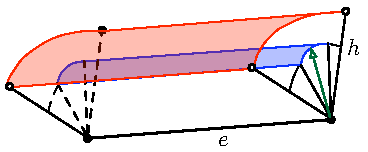
\includegraphics[width=.6\linewidth]{figurefilepath.pdf}
}
\caption{Add an optimal caption.}
\label{fig:name}
\end{figure}

The text in the \s{label} command allows one to refer to the Figure number, in this case I am referring to Figure \ref{fig:name}.  

\section{Macros}
I have included a few simple macros at the top.  For instance use $\Pr[X]$ to indicate the probability of $X$ and use $\E[X]$ to refer to the expected value of $X$.  I usually use a script font $\c{X}$ to refer to a set, for instance $\c{X} = \{X_1, X_2, \ldots, X_n\}$ may indicate a set of $n$ random variables.  

There are lots of other neat math macros built into Latex.  Use dollar signs (e.g. $X_i$) to offset some math text and use slash backets 
\[
M = \sum_{i=1}^n X_i
\]
to use an entire line to write a longer expression.  

\section{More help}
Latex has gotten quite popular, so much so that if you type ``latex'' into google, it lists nothing on the first page about gloves.  

There are some great free references already out there for instance:
\begin{itemize}
\item \url{http://en.wikibooks.org/wiki/LaTeX}
\item \url{http://tex.stackexchange.com/}
\end{itemize}

\end{document}
